

\tikzset{every picture/.style={line width=0.75pt}} %set default line width to 0.75pt        

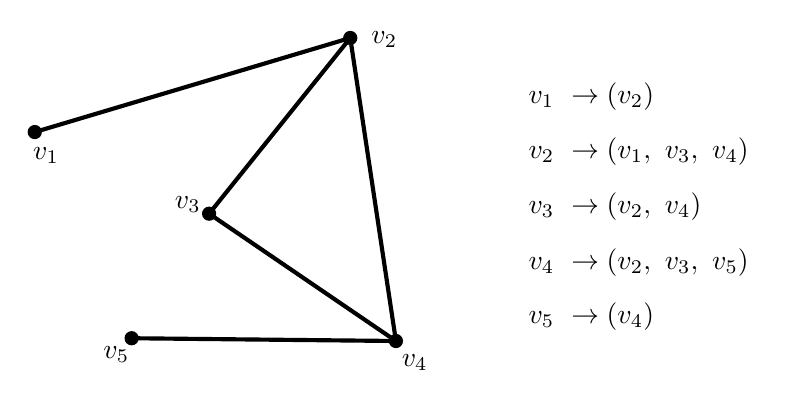
\begin{tikzpicture}[x=0.5pt,y=0.5pt,yscale=-1,xscale=1]
%uncomment if require: \path (0,285); %set diagram left start at 0, and has height of 285

%Flowchart: Connector [id:dp14554034773886415] 
\draw  [fill={rgb, 255:red, 0; green, 0; blue, 0 }  ,fill opacity=1 ] (25,96) .. controls (25,93.58) and (26.96,91.62) .. (29.38,91.62) .. controls (31.79,91.62) and (33.75,93.58) .. (33.75,96) .. controls (33.75,98.42) and (31.79,100.38) .. (29.38,100.38) .. controls (26.96,100.38) and (25,98.42) .. (25,96) -- cycle ;
%Flowchart: Connector [id:dp7796394659617965] 
\draw  [fill={rgb, 255:red, 0; green, 0; blue, 0 }  ,fill opacity=1 ] (253,28) .. controls (253,25.58) and (254.96,23.62) .. (257.38,23.62) .. controls (259.79,23.62) and (261.75,25.58) .. (261.75,28) .. controls (261.75,30.42) and (259.79,32.38) .. (257.38,32.38) .. controls (254.96,32.38) and (253,30.42) .. (253,28) -- cycle ;
%Flowchart: Connector [id:dp8410872532958124] 
\draw  [fill={rgb, 255:red, 0; green, 0; blue, 0 }  ,fill opacity=1 ] (286,247) .. controls (286,244.58) and (287.96,242.62) .. (290.38,242.62) .. controls (292.79,242.62) and (294.75,244.58) .. (294.75,247) .. controls (294.75,249.42) and (292.79,251.38) .. (290.38,251.38) .. controls (287.96,251.38) and (286,249.42) .. (286,247) -- cycle ;
%Flowchart: Connector [id:dp17196535593949425] 
\draw  [fill={rgb, 255:red, 0; green, 0; blue, 0 }  ,fill opacity=1 ] (95,245) .. controls (95,242.58) and (96.96,240.62) .. (99.38,240.62) .. controls (101.79,240.62) and (103.75,242.58) .. (103.75,245) .. controls (103.75,247.42) and (101.79,249.38) .. (99.38,249.38) .. controls (96.96,249.38) and (95,247.42) .. (95,245) -- cycle ;
%Straight Lines [id:da7073971572516686] 
\draw [color={rgb, 255:red, 0; green, 0; blue, 0 }  ,draw opacity=1 ][line width=1.5]    (29.38,96) -- (257.38,28) ;
%Flowchart: Connector [id:dp6372189195472704] 
\draw  [fill={rgb, 255:red, 0; green, 0; blue, 0 }  ,fill opacity=1 ] (151,155) .. controls (151,152.58) and (152.96,150.62) .. (155.38,150.62) .. controls (157.79,150.62) and (159.75,152.58) .. (159.75,155) .. controls (159.75,157.42) and (157.79,159.38) .. (155.38,159.38) .. controls (152.96,159.38) and (151,157.42) .. (151,155) -- cycle ;
%Straight Lines [id:da6054846048754496] 
\draw [color={rgb, 255:red, 0; green, 0; blue, 0 }  ,draw opacity=1 ][line width=1.5]    (155.38,155) -- (257.38,28) ;
%Straight Lines [id:da8238439208450634] 
\draw [color={rgb, 255:red, 0; green, 0; blue, 0 }  ,draw opacity=1 ][line width=1.5]    (99.38,245) -- (290.38,247) ;
%Straight Lines [id:da4336320329770583] 
\draw [color={rgb, 255:red, 0; green, 0; blue, 0 }  ,draw opacity=1 ][line width=1.5]    (290.38,247) -- (257.38,28) ;
%Straight Lines [id:da684522286123465] 
\draw [color={rgb, 255:red, 0; green, 0; blue, 0 }  ,draw opacity=1 ][line width=1.5]    (290.38,247) -- (155.38,155) ;

% Text Node
\draw (26,104.93) node [anchor=north west][inner sep=0.75pt]   [align=left] {$\displaystyle v_{1}$};
% Text Node
\draw (128.38,140.31) node [anchor=north west][inner sep=0.75pt]   [align=left] {$\displaystyle v_{3}$};
% Text Node
\draw (76.75,248.93) node [anchor=north west][inner sep=0.75pt]   [align=left] {$\displaystyle v_{5}$};
% Text Node
\draw (292.38,254.31) node [anchor=north west][inner sep=0.75pt]   [align=left] {$\displaystyle v_{4}$};
% Text Node
\draw (270.38,21.31) node [anchor=north west][inner sep=0.75pt]   [align=left] {$\displaystyle v_{2}$};
% Text Node
\draw (384,58.03) node [anchor=north west][inner sep=0.75pt]   [align=left] {$\displaystyle v_{1} \ \rightarrow ( v_{2})$};
% Text Node
\draw (384,97.78) node [anchor=north west][inner sep=0.75pt]   [align=left] {$\displaystyle v_{2} \ \rightarrow ( v_{1} ,\ v_{3} ,\ v_{4})$};
% Text Node
\draw (384,137.53) node [anchor=north west][inner sep=0.75pt]   [align=left] {$\displaystyle v_{3} \ \rightarrow ( v_{2} ,\ v_{4})$};
% Text Node
\draw (384,178.28) node [anchor=north west][inner sep=0.75pt]   [align=left] {$\displaystyle v_{4} \ \rightarrow ( v_{2} ,\ v_{3} ,\ v_{5})$ \ };
% Text Node
\draw (384,217.03) node [anchor=north west][inner sep=0.75pt]   [align=left] {$\displaystyle v_{5} \ \rightarrow ( v_{4})$};


\end{tikzpicture}

